\documentclass[notheorems,xetex]{beamer}
%\documentclass[UTF8]{ctexbeamer}
\usepackage{xeCJK}%preamble part
%\usepackage{showframe}
\usepackage{amsmath, amsthm, amssymb}
\usepackage{graphicx}
\usepackage{bm}
\usepackage{caption}
\usepackage{ragged2e}
\usepackage{multirow}
\usepackage{float}
\usepackage{color}
\usepackage{listings}
\lstdefinestyle{lstStyleBase}{%
   basicstyle=\small\ttfamily,
   aboveskip=\medskipamount,
   belowskip=\medskipamount,
   lineskip=0pt,
   boxpos=c,
   showlines=false,
   extendedchars=true,
   upquote=true,
   tabsize=2,
   showtabs=false,
   showspaces=false,
   showstringspaces=false,
   numbers=none,
   linewidth=\linewidth,
   xleftmargin=4pt,
   xrightmargin=0pt,
   resetmargins=false,
   breaklines=true,
   breakatwhitespace=false,
   breakindent=0pt,
   breakautoindent=true,
   columns=flexible,
   keepspaces=true,
   gobble=2,
   framesep=3pt,
   rulesep=1pt,
   framerule=1pt,
   backgroundcolor=\color{gray!5},
   stringstyle=\color{green!40!black!100},
   keywordstyle=\bfseries\color{blue!50!black},
   commentstyle=\slshape\color{black!60}}

\lstdefinestyle{lstStyleShell}{%
   style=lstStyleBase,
   frame=l,
   rulecolor=\color{purple},
   language=bash}
%\usepackage[font=Helv,timeinterval=3]{tdclock}
\setbeamertemplate{theorems}[numbered]
\DeclareMathOperator*{\rgmax}{argmax}
\DeclareMathOperator*{\rgmin}{argmin}
\DeclareMathOperator{\tr}{tr}
%\setCJKmainfont{SimSun}[AutoFakeBold=false]
%\setsansfont{SimSun}
\setbeamertemplate{frametitle}[default][center]
\setbeamertemplate{footline}[frame number]
\setlength{\parindent}{0.8cm}
\theoremstyle{definition}
\newtheorem{theorem}{定理}
\newtheorem{lemma}{引理}
\newtheorem{definition}{定义}
\newtheorem{cor}{推论}
%\newcommand{\transpose}[1]{\ensuremath{#1^{\scriptscriptstyle T}}}
\usetheme{Warsaw}
\title{GitHub 高级用法介绍} % (optional, use only with long paper titles)
\author[赵丰]
{\quad {赵丰}\\ \and {zhaofeng-shu33}}
\institute[清华大学] % (optional, but mostly needed)
{\normalsize\quad
  Lab2c 服务器使用培训
}
\date{\the\year 年 \the\month 月 \the\day 日}
%\AtBeginSubsection[]
%{
%  \begin{frame}<beamer>{目录}
%    \tableofcontents[currentsection,currentsubsection]
%  \end{frame}
%}
\usefonttheme[onlymath]{serif}
\setbeamercolor{alerted text}{fg=blue}
\setbeamercolor{normal text}{bg=green!10!white}
\setbeamercolor{frametitle}{fg=blue!50!black,bg=white}
\begin{document}
\frame{\titlepage}
\date{\hspace{1mm} \timemark}
\include{presentation_first_part}
\include{presentation_generalized_continued_fraction}
\section{GitHub 中的个人与组织}
\begin{frame}{GitHub 个人主页}
\begin{itemize}
	\item \url{https://github.com/your_github_id}
	\item 活跃程度
     \begin{figure}
	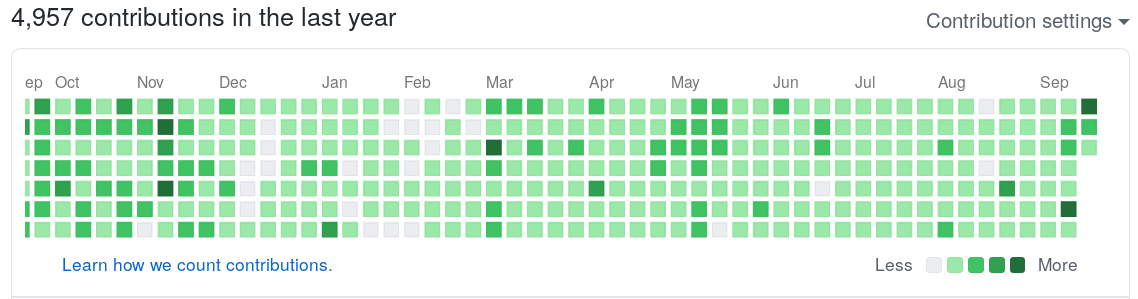
\includegraphics[height=2.5cm]{activity.png}
	\caption*{颜色越深,提交次数越多}
	\end{figure}
	\item 你关注的人与关注你的人
	\begin{figure}
	
\includegraphics[height=1cm]{ff.png}	
	\end{figure}
\end{itemize}
\end{frame}
\begin{frame}{GitHub 组织}
     \begin{figure}
	    \centering
		
\includegraphics[height=2cm]{org.png}
	\end{figure}
\begin{itemize}
	\item 我们的组织 ID: \textbf{mace\_cream}
	\item 置顶的仓库: \textbf{clusterhowto}
	
	\url{https://github.com/mace_cream/clusterhowto}
	\item 接收邀请后,选择自己的可见性: \textbf{公开}或\textbf{仅内部成员可见}。
\end{itemize}
\end{frame}
\begin{frame}[noframenumbering]{如何倒退}
\begin{itemize}
	\item 前提: 经常 commit
	\item 倒退命令
	\begin{enumerate}
		\item [可选]暂存当前修改: \textt{git checkout -b bad\_code}
		\item 回退到想要的地方: \texttt{git reset commit\_hash}
	\end{enumerate}
	\item 
\end{itemize}
\end{frame}
\section{实例分析}
\subsection{merge 中正确解决 conflict}
\begin{frame}[fragile]{merge 中正确解决 conflict}
\begin{itemize}
\item 两个不同的 commit 对同一行代码改动产生了冲突
     \begin{figure}
	\centering
	
\includegraphics[height=0.5cm]{conflict.png}
	\end{figure}
\item 冲突复现
\end{itemize}
\begin{lstlisting}[language=bash]
git clone https://github.com/wuhan2020/\
wuhan2020-frontend-react-app.git
git checkout 801a4e3 -b feature
git checkout 9d11a11 -b main
git merge feature
\end{lstlisting}

\end{frame}
\begin{frame}{冲突现象}

\begin{figure}
	\centering
	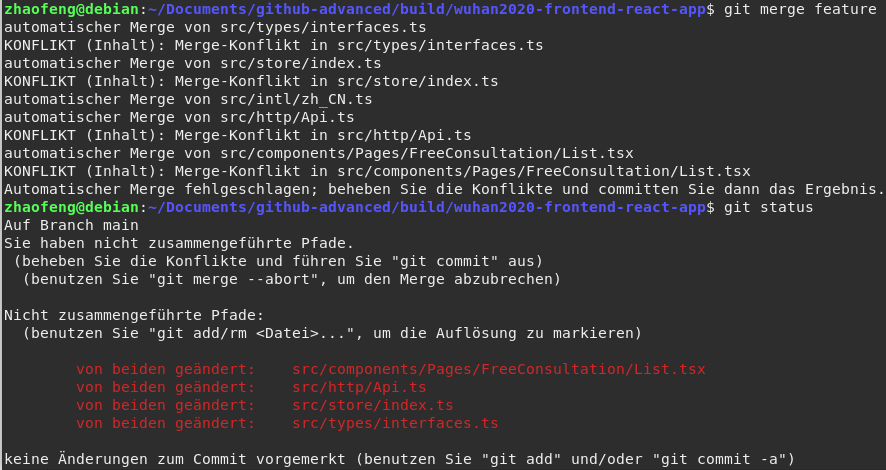
\includegraphics[height=6cm]{phenomenon.png}
\end{figure}
\end{frame}
\begin{frame}{冲突原因}
\begin{figure}
	\centering
	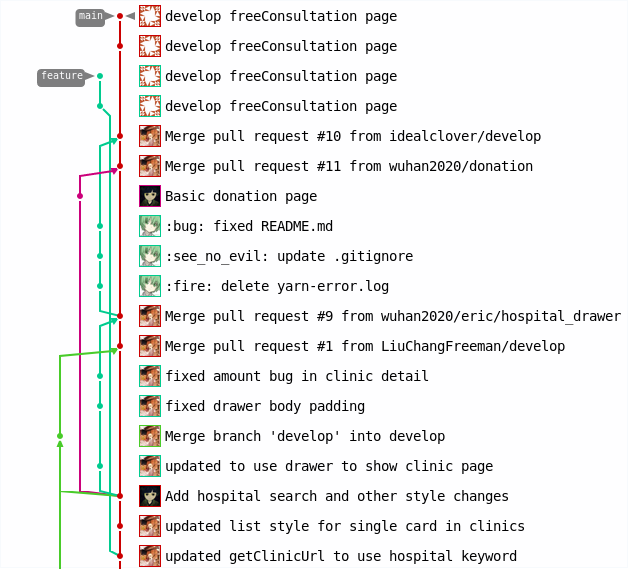
\includegraphics[height=7cm]{deps.png}
\end{figure}
\end{frame}
\begin{frame}{如何解决}
\begin{itemize}
	\item 使用 IDE 工具选择接受哪一部分的改动
\end{itemize}
\begin{figure}
	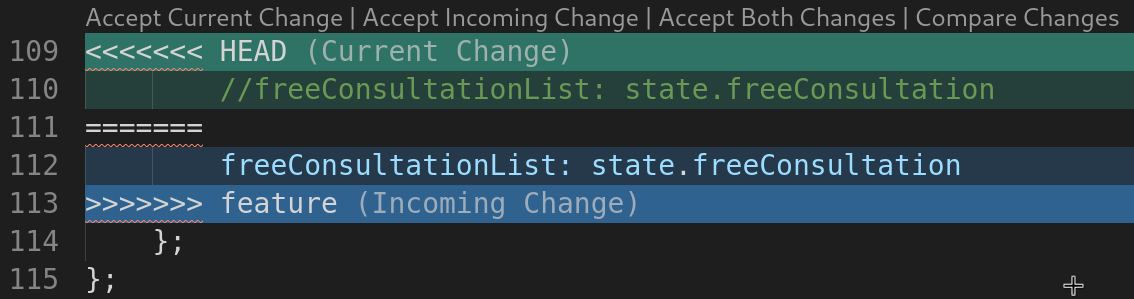
\includegraphics[height=2.5cm]{accept_incoming.png}
\end{figure}

\end{frame}
\begin{frame}{最终效果}
\begin{figure}
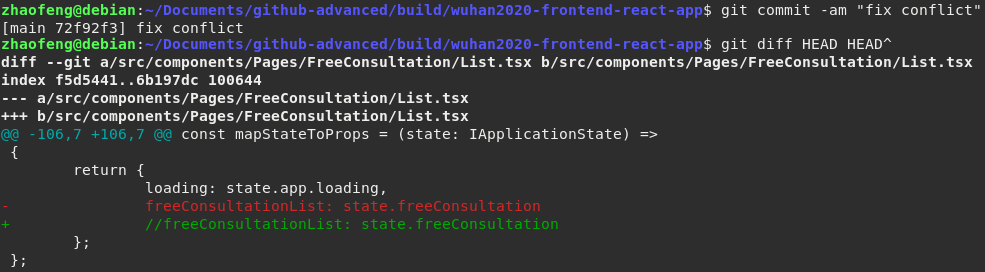
\includegraphics[height=2.5cm]{recover_changes.png}
\caption{复现效果}
\end{figure}
feature 分支仅贡献一处改动
\begin{figure}
	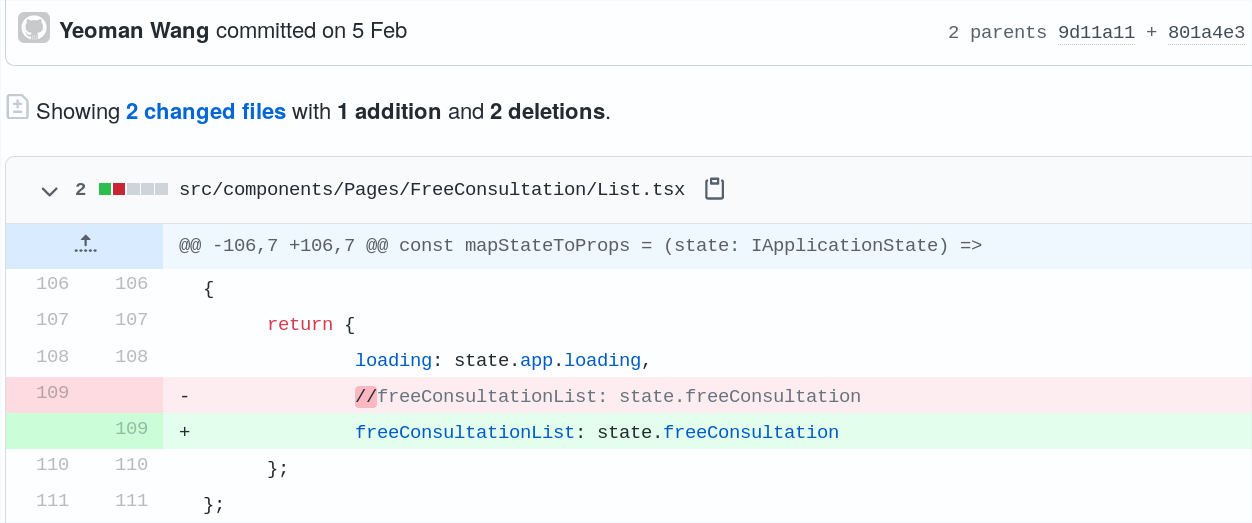
\includegraphics[height=2.5cm]{original.png}
	\caption{原有效果}
\end{figure}
\end{frame}


\begin{frame}[noframenumbering]{如何使用 tag}
提取公因子后,下面用连分式法研究$\bm{I}(\bm{P})=\lambda \bm{I}+\bm{J}$的结构。
\pause
$t_{i}$时刻的位置信息椭圆为
\[
\bm{e}_{i}^{\textrm{T}}(\bm{I}(\bm{P}))^{-1}\bm{e}_{i}
\]
其中
\begin{equation*}
\bm{e}_i=(\bm{0},\dots,\underbrace{\bm{I}_2}_{i\text{-th item}},\dots,\bm{0})^{\textrm{T}}.
\end{equation*}
\end{frame}
\begin{frame}[noframenumbering]
$\bm{I}(\bm{P})$可以简写为:
\begin{equation*}
\bm{I}(\bm{P})=\begin{pmatrix}
                 \bm{B}_1 & \bm{A}_2 & \bm{0} & \dots & \bm{0} \\
                 \bm{A}_2 & \bm{B}_2 & \bm{A}_3 & \dots & \bm{0} \\
                 \vdots & \vdots & \vdots & \ddots & \vdots \\
                 \bm{0} & \dots & \bm{0} & \bm{A}_{N_a} & \bm{B}_{N_a}
               \end{pmatrix}.
\end{equation*}

$\bm{I}(\bm{P})$可以做LU分解如下:
\pause
\begin{equation*}\label{eq:LU}
  \bm{I}(\bm{P})=\begin{pmatrix}
                 \bm{I}_2 & \bm{0} & \bm{0} & \dots & \bm{0} \\
                 \bm{L}_2 & \bm{I}_2 & \bm{0} & \dots & \bm{0} \\
                 \vdots & \vdots & \vdots & \ddots & \vdots \\
                 \bm{0} & \dots & \bm{0} & \bm{L}_{N_a} & \bm{I}_{2}
               \end{pmatrix}\begin{pmatrix}
                 \bm{U}_1 & \bm{A}_2 & \bm{0} & \dots & \bm{0} \\
                 \bm{0} & \bm{U}_2 & \bm{A}_3 & \dots & \bm{0} \\
                 \vdots & \vdots & \vdots & \ddots & \vdots \\
                 \bm{0} & \dots & \bm{0} & \bm{0} & \bm{U}_{N_a}
               \end{pmatrix}.
\end{equation*}
\end{frame}
\begin{frame}[noframenumbering]
$\bm{U}_i$满足如下递推关系:
\begin{equation*}
\begin{cases}
  \bm{U}_1 &= \bm{B}_1 \\
  \bm{U}_i &= \bm{B}_i-\bm{A}_i\bm{U}_{i-1}^{-1}\bm{A}_i,i\geq 2.
\end{cases}
\end{equation*}

其中
\begin{equation*}
\begin{cases}
  \bm{A}_i &= -\bm{u}_i\bm{u}_i^{\textrm{T}} \\
  \bm{B}_i &=\lambda\bm{I}_2+\bm{u}_{i-1}\bm{u}_{i-1}^{\textrm{T}}+\bm{u}_i\bm{u}_i^{\textrm{T}}, 2 \leq i \leq N_a-1.
\end{cases}
\end{equation*}
\end{frame}
\begin{frame}[noframenumbering]
\begin{equation*}\label{eq:LU}
  \bm{I}(\bm{P})=\begin{pmatrix}
                 \bm{I}_2 & \bm{0} & \bm{0} & \dots & \bm{0} \\
                 \bm{L}_2 & \bm{I}_2 & \bm{0} & \dots & \bm{0} \\
                 \vdots & \vdots & \vdots & \ddots & \vdots \\
                 \bm{0} & \dots & \bm{0} & \bm{L}_{N_a} & \bm{I}_{2}
               \end{pmatrix}\begin{pmatrix}
                 \bm{U}_1 & \bm{A}_2 & \bm{0} & \dots & \bm{0} \\
                 \bm{0} & \bm{U}_2 & \bm{A}_3 & \dots & \bm{0} \\
                 \vdots & \vdots & \vdots & \ddots & \vdots \\
                 \bm{0} & \dots & \bm{0} & \bm{0} & \bm{U}_{N_a}
               \end{pmatrix}.
\end{equation*}

从上式可以求出
\begin{equation*}\label{eq:thomas_final}
\bm{e}_{N_a}^{\textrm{T}}(\bm{I}(\bm{P}))^{-1}\bm{e}_{N_a}=U_{N_a}^{-1}.
\end{equation*}
\pause

关于$U_{N_a}$的结构我们有结论,它的一个特征值是$\lambda$,另一个特征值可以用连分式表示出来。
\end{frame}
\begin{frame}[noframenumbering]
设$\bm{u}_i=(\cos\theta_i,\sin\theta_i)^{\textrm{T}}$
\begin{equation*}
\begin{split}
T_{i-1} =& \lambda + \frac{1}{1+\frac{\sin^2\theta_i}{\lambda}+\frac{\cos^2\theta_i}{T_i}},2\leq i\leq N_a-1\\
T_{N_a-1}  =& \lambda+\frac{1}{1+1/\lambda}
\end{split}
\end{equation*}

$T_1$就是$U_{N_a}$的另一个特征值。
\end{frame}
\begin{frame}[noframenumbering]{GitHub Action}
可以用归纳法得到
\[
[\lambda,1,\underbrace{\lambda,1}_{\text{$n$ item}}]=\frac{P_{n+1}(\lambda)}{Q_n(\lambda)}
\]
其中$P_{n+1}(\lambda),Q_n(\lambda)$是关于$\lambda$的n+1和n次多项式。
\end{frame}
\begin{frame}[noframenumbering]
有理分式逼近(Pad\'{e}逼近)理论指出对于光滑函数$f(x)$,可构造有理分式:
\[
R_{n+m}(x)=\frac{P_n(x)}{Q_m(x)}
\]
来逼近$f(x)$,使得$R_{n+m}(x)$与$f(x)$在$x=0$处直到$n+m$次导数相等。
\pause


Taylor级数是$m=0$的情形
\pause

函数的有限连分式展开在某些情况下是$|n-m|=1$的情形
\begin{flushright}
\hspace{ \stretch{1} }\fbox{\parbox[b][5em][t]{0.4\textwidth}{Pad\'{e} approximation and continued fractions, Applied Numerical Mathematics, 2010}}
\end{flushright}
\end{frame}
\begin{frame}[noframenumbering]
下面我们考虑$m+n$相等时不同的展开方式对$f(\lambda)=\frac{\lambda+\sqrt{4\lambda+\lambda^2}}{2}$逼近的效果情况,
\pause

由于$f(\lambda)$在$\lambda=0$处有奇性(一阶导数不存在),我们考虑其在复平面关于$\infty$的Taylor展开式,通过令$x=1/\lambda$不难得到
\begin{align}\notag
f(\lambda)=&\frac{2}{\sqrt{1+4x}-1}\\
=&\frac{1}{x-x^2+2x^3-5x^4+14x^5+\dots}
\end{align}

由于$\sqrt{1+4x}$收敛域为$|4x|<1$可得$|\lambda|>4$,可见Taylor展开对$\lambda$的取值有限制。
\end{frame}
\begin{frame}[noframenumbering]
\begin{figure}
\centering
\caption*{取n+m=5对$f(\lambda)$的有理逼近图示}
%\includegraphics[width=300pt]{pade.eps}
\end{figure}
\begin{itemize}
  \item Taylor展开逼近在$\lambda<4$时偏离较大
  \item pade41收敛域大于Taylor展开,但在$\lambda$较小处仍然不收敛
  \item 连分式对应的pade32对于$\lambda>0$逐点收敛到$f(\lambda)$
\end{itemize}
\end{frame}

%\subsection{正方形网络和正六边形网络}
%\begin{frame}[noframenumbering]
%在正方形网络中,由于正交性,定位效果并不理想。
%  \begin{columns}[T] % contents are top vertically aligned
%     \begin{column}[T]{6cm}
%     右图中$\bm{p}_3$的位置信息要想被$\bm{p}_1$利用提高定位精度,是通过改善$\bm{p}_2$的定位精度间接实现的。
%     \pause
%但是$\bm{p}_3$对$\bm{p}_2$位置精度的贡献的方向恰好与$\bm{p}_2$对$\bm{p}_1$位置精度的贡献的方向垂直,因此$\bm{p}_3$对$\bm{p}_1$定位精度的提高没有贡献。
%     \end{column}
%     \begin{column}[T]{5cm} % alternative top-align that's better for graphics
%          \includegraphics[height=4cm]{orthogonal.eps}
%     \end{column}
%     \end{columns}
%\end{frame}
%\begin{frame}[noframenumbering]
%在正六边形网络中,类似线性网络中的直接法,
%通过采用节点分层技术可以得到网络规模趋向于无穷大时的节点平均定位误差下界为
%  \begin{equation}
%  \lambda+\frac{3}{2}-\cfrac{3/2}{\lambda+\frac{3}{2}-\cfrac{1/2}{\lambda+3/2-\dots}}=\sqrt{\lambda^2+3\lambda+\frac{1}{4}}-\frac{1}{\lambda+\frac{3}{2}+\sqrt{\lambda^2+3\lambda+\frac{1}{4}}}.
%  \end{equation}
%\end{frame}
%\begin{frame}[noframenumbering]
%  在数学方法方面,本文主要的成果如下:
%  \begin{itemize}
%  \item
%    使用复数表示法推导得出非协作定位场景下费舍尔信息矩阵的特征值和特征向量的表达式。
%  \item
%    推导得出秩一矩阵的克罗内克积对N维对称正定矩阵扰动后行列式的表达式。
%  \item
%    推导得出二维场景下特殊完全图的邻接矩阵所有特征值,其中使用瑞利商给出了最大 特征值的表达式。
%  \item 推导得出二维场景下特殊度为2的图的邻接矩阵的所有特征值;当网络规模趋向无穷大时,求出了所有特征值的倒数和的平均值的极限。
%  \item 使用连分式推导得出形如$\lambda \bm{I}+\bm{J}$的对称正定矩阵$\bm{A}$确定的$\bm{A}^{-1}_{1\times2,1\times2}$的两个特征值;分析得出了决定特征值的连分式的序列指数收敛的特性,并做出适当的推广。
%  \end{itemize}
%
%\end{frame}
%\begin{frame}[noframenumbering]
% \frametitle{参考文献}
% \tiny
% \begin{itemize}
%   \item Kegen Yu I S, Guo Y J. Ground-Based Wireless Positioning. John Wiley and Sons, Ltd,2009
%   \item L J, S L, G V. Development and experimental validation of an adaptive extended kalman filter for the localization of mobile robots. IEEE Transactions, 1999, 15(2):219–229
%   \item Shen Y, Win M Z, Wymeersch H. Fundamental limits of wideband localization—part
%i: A general framework. IEEE TRANSACTIONS ON INFORMATION THEORY, 2010,
%56(10):4956–4980
%   \item 杨思怡. 协作定位网络的信息耦合机理 [D]. 北京: 清华大学, 2016
%   \item 姚慕生. 高等代数学. 上海: 复旦大学出版社, 2003
%   \item MazuelasS,ShenY,WinMZ. Spatio-temporalinformationcouplingincooperativenetwork
%navigation. Globecom Communication Theory Symposium, 2012. 2403–2407
%   \item 关治, 陆金甫. 数值分析基础. 北京: 高等教育出版社, 2010: 52–56
%   \item Hammond W F. Continued fractions and the euclidean algorithm. Lecture notes, University
%at Albany, 1997
% \end{itemize}
%\end{frame}

\end{document}